\chapter
    [Structural Subtyping: The Static Soul of Dynamic Languages]
    {Structural Subtyping: \newline The Static Soul of Dynamic Languages}
\label{static-soul}

This chapter both builds the motivation of this thesis, and introduces various key concepts -- such as nominal or structural (sub)typing -- that arise throughout the report.

We begin by exploring characteristics of dynamically typed programs that we might like to type statically (Section \ref{sec:background}). I~propose for \textbf{duck typing} to be the key characteristic we should focus our attention on, and argue that \textbf{structural subtyping} is a solid approach for statically modelling this pattern. Afterwards, via the introduction of a \emph{translation} in Section \ref{sec:translations}, I ground intuitions about structural subtyping and its expressivity.

\section{Background}
\label{sec:background}

We first consider the meaning of \emph{dynamic} and \emph{static} typing.

\emph{Dynamic typing} generally means any form of runtime type checking, while \emph{static typing} is type checking at compile time. A dynamically typed language (or program) relies only on dynamic typing, and not static typing. Since when we talk about \emph{typing} we generally mean static typing, we also call dynamically typed programs \emph{untyped}.\todo[color=red]{really untyped?} 

Many statically typed languages possess some facilities for dynamic type checking, blurring the line between static and dynamic languages: \begin{description}
    \item[Static can be dynamic] Java (along with many other object-oriented languages) features \textit{downcasts}, which coerce an object of some class into its subclass. This has to be checked at runtime to preserve safety. 
    % It would be entirely possible -- though impractical -- to program in Java using only the \texttt{Object} type and to rely on downcasts for any useful work, essentially circumventing static typing. 
    More glaringly, Java also has reflection facilities, allowing introspection of types of values at runtime. 
    \item[Dynamic can be static] Most dynamically typed languages \emph{could} be given a trivial static type system (c.f.\@ the wildcard/any type). 
    % for instance, determining whether a given piece of code is a statement (of type \textsf{stmt}), or expression (of type \textsf{value})
    Checking such types would be entirely syntax-directed.
\end{description} 

Furthermore, the line between type checking and other kinds of checks is itself subjective.
Verifying that an index into an array is an integer is obviously known to be type checking.
On the other hand, determining whether the index is out-of-bounds is generally thought not to be a type check -- even though it is handled as such in a dependent type system. 

Hence, it is difficult say what dynamic language patterns we should attempt to type statically, and what type safety properties we should ensure. It is necessary to make some assumptions in order to proceed further.
After all, the space of dynamically typed programs is extremely large -- but there are only so many interesting patterns hiding within.

\needspace{6em}
\subsection{Taming runtime type checking}
\label{subsec:runtime-type-checking}

Let us distinguish two kinds of runtime type checking -- with the goal of identifying a well-behaving subset: \begin{description}
    \item[Types as data] A value's type can be read and itself operated on as a value. For example, both Python and Lua feature a \texttt{type} built-in function. Since the type becomes a runtime value, it can arbitrarily affect the data and control flow. 
    Branching on the type (e.g.\@ Python's \texttt{isinstance}) -- a common pattern in literature on \emph{set-theoretic types} -- also treats the type as data. 
    
    I exclude the principle of types as data, as it has the following conseqeuences: \begin{description}
        \item[Lack of \emph{parametricity}] -- accessing the type of a value is always legal, i.e. it is of type $\forall \alpha \ldotp \alpha \to \textsf{Type}$. However, since the type directly impacts the result of the computation, \emph{parametricity} no longer holds: it is no longer the case a parametrically-polymorphic function performs the same computation in any type instantiation. This stops us from enjoying useful properties -- like theorems for free \cite{theorems-for-free} -- and leads to the second point.
        \item[Lack of \emph{predictability}] -- Subjectively speaking, code using types as data is more complicated and confusing to follow. This is reflected in any attempt to statically analyse them -- even when we limit ourselves to branching on types, it is known that we are limited computationally by the need for \emph{backtracking} \cite{polymorphic-set-theoretic-types}.
    \end{description}
    \item[Types as runtime guardrails] A value's type could instead be consulted only when we perform an operation on it, in order to check whether the operation is legal -- with an error raised otherwise -- similarly to how types are used in statically typed languages.     
    
    For example, consider a \emph{record} (or \emph{object}) data type, which stores some list of labelled fields, and is commonly featured in dynamic languages. 
    We usually consider the labels of fields present to be part of the record's type.
    Accessing a field of an object requires a (dynamic \emph{or} static) type check for whether it is present in the object.
    
    Viewing types as guardrails -- sources of merely runtime type errors, and not information about a value -- follows the \textbf{duck typing} pattern \cite{duck-typing} of untyped programs. If we expect an object to \texttt{quack()}, then we worry about nothing else but for our program to \texttt{quack()}. This embodies the principle \textit{\enquote{ask for forgiveness, not permission}}.
    % -- programs assume that all operations are legal.
    Note that -- provided we do not handle errors raised due to illegal operations -- duck typing does not suffer from the same loss of parametricity.
\end{description}
I thus chose to design an approach to static typing which admits programs utilising \textbf{duck typing} -- motivated by the fact that it preserves parametricity. 
We now have to find a way to statically model duck typing.

\subsection{Modelling duck typing}
\label{subsec:duck-models}

Having identified duck typing as a crucial well-behaved pattern in dynamically-typed programs, it remains to find its \emph{static soul} -- a method which admits a corresponding pattern, but can be statically typed.

\subsubsection{Structural subtyping}

Duck typing naturally admits a natural notion of \textbf{subtyping}: if a duck $a$ of type $A$ quacks, and another duck $b$ of type $B$ not only quacks but also walks -- then clearly $b$ can be used in any place $a$ can. A substitution principle holds: the type $B$ supports more operations than $A$, and thus $B$ is a subtype of $A$ -- we shall denote this $A \sub B$. When speaking of subtyping, we usually refer to its \emph{implicit} variety -- the language does not require an \emph{explicit} annotation every time we treat a type as its supertype.

This is a good time to introduce a distinction between \textbf{nominal} and \textbf{structural} (static) typing \cite{pierce-book}. \begin{description}
    \item[Nominal] Most static type systems in popular programming languages are nominal: types are introduced via a type definition, where they are \emph{named} -- the type is then identified with (e.g.\@ compared by) this name. For example, the type systems in Java, C/C++, and Haskell are predominantly nominal.
    \item[Structural] On the other hand, a structural type system does not pose the requirement for a type to have a name nor a definition. A popular example of a structurally typed language would be TypeScript -- the statically typed dialect of JavaScript. 
\end{description}
Similarly to static and dynamic, nominal and structural typing also lie on a spectrum: few languages feature solely nominal or structural types. A good example of a language with a mix of nominal and structural typing is OCaml (Figure \ref{fig:nominal-and-structural-ocaml}): while records and variants can only be introduced in a \emph{nominal} type definition, we can introduce \emph{structural} type abbreviations. In particular, we have structural versions of records (objects) and variants (polymorphic variants). OCaml modules are structurally typed, too.

\begin{figure}
    \centering
    \begin{subfigure}{.49\textwidth}
    \centering
    \begin{ocaml}
(* record *)
type point = { x : int; y : int }
(* variant *)
type opt = None | Some of int
    \end{ocaml}
    \caption{Nominally typed records and variants.}
    \label{subfig:nominal-ocaml}
    \end{subfigure}
    \hfill
    \begin{subfigure}{.49\textwidth}
    \centering
    \begin{ocaml}
(* object *)
type point = < x : int; y : int >
(* polymorphic variant *)
type opt = [ `None | `Some of int ]
    \end{ocaml}
    \caption{Structurally typed objects and polymorphic variants.}
    \label{subfig:structural-ocaml}
    \end{subfigure}
    \caption{Examples of nominal and structural type definitions in OCaml. Note that the same syntax is used for both nominal type definitions (Figure \ref{subfig:nominal-ocaml}) and structural type abbreviations (Figure \ref{subfig:structural-ocaml}), even though these two kinds of type declarations behave differently in OCaml's type system.}
    \label{fig:nominal-and-structural-ocaml}
\end{figure}

Intuitively, a nominally typed program can be transformed into a structurally typed one, and as such structurally typed programs are inherently more flexible -- we explore this in Section \ref{sec:translations}. 
% This fundamental idea of \emph{anonymising types} by erasing their names is formally explored in the \textbf{translations} presented in Section \ref{sec:translations} on the languages we introduce in Section \ref{sec:languages}.

We also introduce a similar distinction between nominal and structural \textbf{subtyping}: while in a language like Java subtyping is defined through the inheritance hierarchy (\texttt{class C extends C' \{ ... \}}) -- subtyping is defined on types with specific names -- structural subtyping is instead defined in terms of the structure of the type. Structural subtyping naturally arises on records (and, dually, variants) through the following two rules:\footnote{A traditional formal treatment is given by \textcite{pierce-book}. In this dissertation -- to express it more conveniently for algebraic subtyping in Chapter \ref{algebraic-subtyping} -- we use a slightly different approach with \emph{field types}.}
\begin{description}
    \item[Width subtyping] A record is a subtype of another if it has more fields and the other are compatible, e.g.: $$ \{ \mathrm{foo} : \mathrm{int}, \mathrm{bar} : \mathrm{string} \} \sub \{ \mathrm{foo} : \mathrm{int} \} $$
    \item[Depth subtyping] A record is a subtype of another if its respective fields are subtypes, e.g.:
    $$ \{ \mathrm{foo}: \mathrm{nat}, \mathrm{bar}: \mathrm{string} \} \sub \{ \mathrm{foo}: \mathrm{int}, \mathrm{bar}: \mathrm{string} \} $$
\end{description}

We formalise this in the type system for the record calculus -- Featherweight Lua -- in Section~\ref{subsec:featherweight-lua}.

Clearly, \textbf{structural subtyping} is most relevant for modelling duck typing: most dynamically typed programs will not feature type definitions.\footnote{A note-worthy exceptions would be OOP-style class definitions, present in e.g.\@ Python.} I am mainly motivated by modelling objects in dynamic languages, following the tradition of \textcite{cardelli-multiple-inheritance}.

I chose structural subtyping as the direction for my thesis -- we briefly consider two possible alternatives in the following subsections. I motivate this mainly choice by the recency of the seminal work of \textcite{mlsub} on \emph{algebraic subtyping} -- the topic of Chapter \ref{algebraic-subtyping} -- as it is directly applicable to languages with certain forms of structural subtyping.

\subsubsection{Row polymorphism}

\begin{figure}
    \centering
    \begin{tabular}{c}
    \begin{ocaml}
let f = function 
    | `None -> `Unit 
    | `Some x when x mod 2 = 0 -> `Pair (x / 2, x / 2) 
    | `Some x -> `Single x
(* 
val f : [< `None | `Some of int ] 
     -> [> `Pair of int * int | `Single of int | `Unit ]
*)
    \end{ocaml}
    \end{tabular}
    \caption{Example of row polymorphism in OCaml using polymorphic variants, annotated with its (inferred) most general type. \texttt{<} and \texttt{>} stand for row type variables in a closed and open variant, respectively. The argument type can be unified against any variant with at most the listed cases, while the result with at least those.}
    \label{fig:ocaml-row-polymorphism}
\end{figure}

There is a common folklore trick for replacing subtype polymorphism -- as seen for objects/records above -- by an appropriate form of parametric polymorphism \cite{structural-subtyping-as-parameric-polymorphism}. For example, a function of type $\top \to \mathrm{int}$ -- featuring a top type $\top$, the supertype of any type -- could equivalently be given the type scheme $\forall \alpha \ldotp \alpha \to \mathrm{int}$, since $\alpha$ can be instantiated to any argument type.
\textbf{Row polymorphism} \cite{remy-records}, introduced by \textcite{wand-rows} (more generally \emph{structural polymorphism} \cite{simple-structural-polymorphism}) -- can be seen as an application of this trick to structural record and variant types: we introduce \emph{row type variables} that stand for \enquote{the rest of the record}.
% Width subtyping correspond to instantiation of row variables, while depth subtyping corresponds to nested instantations.

% https://ocaml.org/papers
% https://brianmckenna.org/blog/row_polymorphism_isnt_subtyping
A technical explanation of row polymorphism is outside the scope of this thesis, so we focus on the practical example of OCaml's objects \cite{objective-ml} and polymorphic variants \cite{polymorphic-variants} -- as exemplified in Figure \ref{subfig:structural-ocaml}. These are typed using row polymorphism with \emph{implicit} row variables \cite{objective-ml}, which can cause some awkward limitations \cite{castagna-polymorphic-variants}. OCaml also supports \emph{explicit} (super)type coercions anyhow, adding a form of explicit structural subtyping -- managing the limitations of the row polymorphism design. 
An example application of row polymorphism in OCaml is given in Figure \ref{fig:ocaml-row-polymorphism}.

The relative power of structural subtyping and row polymorphism -- as extensions on parametric polymorphism -- is unclear.
% , and building systems based on row polymorphism is a viable alternative -- though possibly limited in the context of types for which rows are not clearly helpful in modelling notions of subtyping. 
There is some recent work exploring the relationship between the two \cite{disjoint-polymorphism, structural-subtyping-as-parameric-polymorphism}. However, systems with row polymorphism tend to grow more complex than ones with subtyping \cite{castagna-polymorphic-variants}. Nonetheless, they have historically been a feasible extension of ML-like type systems.

\subsubsection{Set-theoretic types}

With \textbf{set-theoretic types}, we extend the type language with operators corresponding to set operations:
$$ \tau ::= \cdots \mid \tau \cup \tau \mid \tau \cap \tau \mid \lnot \tau $$
These operators admit a set-theoretic interpretation -- they are exactly compatible with the sets of expressions (values) that have a given type $\tau$. 
Under this interpretation, the set-inclusion relation naturally gives us a notion of subtyping, so that e.g.\@ $\tau \cap \tau' \sub \tau'$.
Set-theoretic types are elegant, expressive, and have seen practical use \cite{set-theoretic-types-for-elixir, set-theoretic-types-for-erlang}. However, it is difficult to efficiently infer and simplify them, and type inference usually lacks \emph{principal types}, enjoyed by ML-style type inference -- like algebraic subtyping \cite{mlstruct, castagna-dynamic}. 

Later, in algebraic subtyping\todo[color=green]{move?} -- a technique that builds on structural subtyping -- we rely on a type lattice construction featuring meets $\meet$ (least upper bounds) and joins $\join$ (greatest lower bounds). Though similar at first sight, the two approaches are subtly different \cite{mlstruct}: while $(\mathrm{int} \to \mathrm{int}) \cup (\mathrm{nat} \to \mathrm{nat})$ is as valid a type as any other, in the type lattice of MLsub \cite{mlsub} and MLstruct \cite{mlstruct} we have: $$(\mathrm{int} \to \mathrm{int}) \join (\mathrm{nat} \to \mathrm{nat}) = (\mathrm{int} \meet \mathrm{nat} \to \mathrm{int} \join \mathrm{nat}) = \mathrm{nat} \to \mathrm{int} $$
While $\cup$ gives us a function type which preserves its argument's type, $\join$ only grants that the function must accept $\mathrm{nat}$ and only returns $\mathrm{int}$ (cf.\@ subtyping of functions).
Hence, types no longer have a direct set-theoretic interpretation.\footnote{Note that type lattices exist where the equation does not hold, and that Dolan's system admits some set-theoretic-esque types like $\{\} \meet (\top \to \top)$ (though they can only be used as $\top$) where necessary for \emph{extensibility}.} It thus seems that set-theoretic types are no less expressive than approaches based on algebraic subtyping, where types are constrained to just the ones in the defined lattice. To the author's knowledge, no formal relationship between the two has been established.

\section{Languages}
\label{sec:languages}

As I have now determined the main approach to static typing in this thesis -- \textbf{structural subtyping} -- we are in need of some initial model languages to ground any further conclusions.

Firstly, I construct a simple calculus, which I dub \textbf{Featherweight Lua} (FL), that we will use to model a dynamically typed language with a statically typed fragment featuring structural subtyping. As the name implies, FL admits a simple embedding into its namesake, the popular dynamically typed language Lua. Secondly, I recall the established \textbf{Featherweight Java} (FJ) calculus, and use it as a model for a nominally typed OOP language.  

\subsection{Featherweight Lua}
\label{subsec:featherweight-lua}

I construct FL as the simply-typed lambda calculus extended with extensible record types. Expressions and types in FL are given in Figure \ref{fig:featherweight-lua-grammar}. We consider key aspects in the following subsections.

\begin{figure}
    \centering
    \begin{subfigure}{.49\textwidth}
\begin{align*}
    \graintro e
    x 
    & \text{(variable)}
    \graitem
    \fllet{x}{e}e
    & \text{(let-binding)}
    \graitem
    \fllam{x} e
    & \text{(function)}
    \graitem
    e\,e
    & \text{(application)}        
    \graitem
    \flrec{\overline{\ell = e}}
    & \text{(record construction)}
    \graitem
    \flext{\ell = e}{e}
    & \text{(record extension)}
    \graitem
    \flproj{e}{\ell}
    & \text{(record projection)}
    \graitem
    \flcast{e}{\tau}
    & \text{(subtype coercion)}
    \\ \\
    \graintro v
    \fllam{x} e
    & \text{(function)}
    \graitem
    \flrec{\ell = v}
    & \text{(record)}
\end{align*}
\caption{Expressions $e$ and values $v$ in Featherweight Lua.}
\label{fig:featherweight-lua-expr}
\end{subfigure}
\hfill
\begin{subfigure}{.49\textwidth}
\begin{align*}
    \graintro \tau
    \tau \to \tau
    & \text{(function)}
    \graitem
    \flext{\overline{\ell : \phi}}{\phi}
    & \text{(record)}
    \\ \\ 
    \graintro \phi 
    \top
    & \text{(top)}
    \graitem
    \bot 
    & \text{(bottom)}
    \graitem
    \tau
    & \text{(present)}
    \graitem
    \flabsent 
    & \text{(absent)}
\end{align*}
$$ \flrec{ \overline{\ell : \tau_\ell} } \defeq \flrec{ \overline{\ell : \tau_\ell} \mid \top } $$
\caption{Types $\tau$ and field types $\phi$.}
\label{fig:featherweight-lua-types}
\end{subfigure}

    \caption{Syntax of Featherweight Lua.}
    \label{fig:featherweight-lua-grammar}
\end{figure}

\subsubsection{Expressions}

Since FL's functions and bindings are entirely standard, we consider its records and coercions:\todo{opsem?}
\begin{description}
    \item[Records] Records can be constructed from a list of individual assignments, and individual fields can be projected. Since FL's records are extensible, we have a record extension operator, which, given an existing record without an assignment to a field, returns a new record with that field set.
    \item[Coercion] FL features a type coercion operator, which is a no-op at runtime. It is included as it plays a role in the FJ-FL translation later.
\end{description}

\subsubsection{Typing}

\begin{figure}
    \centering
    $$ 
\begin{array}{c}
\flproj{\tau}{\ell} \defeq \begin{cases}
    \phi_\ell, & \ell \text{ occurs in } \tau \\
    \phi, & \ell \text{ does not occur in } \tau
\end{cases} \qquad \text{where } \tau = \flext{ \overline{\ell : \phi_\ell}}{\phi}
\\[1.5em]
\boxed{\tau \sub \tau}
\\[0.5em]
\irule{FL-Sub-Fun}{\tau_1 \super \tau_2 \quad \tau_1' \sub \tau_2'}{\tau_1 \to \tau_1' \sub \tau_2 \to \tau_2'}
\qquad
\irule{FL-Sub-Rec}{\forall \ell \in \mathcal L(\tau_1) \cup \mathcal L(\tau_2) \ldotp \flproj{\tau_1}{\ell} \sub \flproj{\tau_2}{\ell}}{\tau_1 \sub \tau_2}
\\[2.5em]
\boxed{\phi \sub \phi}
\\[1em]
\flfbot \sub \tau \sub \flftop \qquad \flfbot \sub \flabsent \sub \flftop
\end{array} 
$$
    \caption{Declarative definition of the subtyping relation $\sub$ in Featherweight Lua, including on field types $\phi$. $\mathcal L(\tau)$~stands for the set of labels $\ell$ in the record type $\tau$. We define projection on record types,~$\flproj{\tau}{\ell} = \phi.$}
    \label{fig:featherweight-lua-subtyping}
\end{figure}

\begin{figure}
    $$ 
\begin{array}{c}
\boxed{\Gamma \vdash e : \tau} 
\\[0.5em]
\Gamma ::= \cdot \mid \Gamma, x : \tau
\\[1em]
\irule{FL-Typ-Var}{\Gamma(x) = \tau}{\Gamma \vdash v : \tau}
\quad 
\irule{FL-Typ-Sub}{\Gamma \vdash e : \tau \quad \tau \sub \tau'}{\Gamma \vdash e : \tau'}
\quad
\irule{FL-Typ-Cast}{\Gamma \vdash e : \tau}{\Gamma \vdash \flcast e \tau' : \tau'}
\\[2em]
\irule{FL-Typ-Let}{\Gamma \vdash e : \tau \quad \Gamma, x : \tau \vdash e' : \tau'}{\Gamma \vdash \fllet{x}{e}{e'} : \tau'}
\quad 
\irule{FL-Typ-Fun}{\Gamma, x : \tau \vdash e : \tau'}{\Gamma \vdash \fllam{x} e : \tau \to \tau'}    
\quad 
\irule{FL-Typ-App}{\Gamma \vdash e : \tau' \to \tau \quad \Gamma \vdash e' : \tau'}{\Gamma \vdash e\,e' : \tau}
\\[2em]
\irule{FL-Typ-Cons}
    {\overline{\Gamma \vdash e_\ell : \tau_\ell}}
    {\Gamma \vdash \flrec{\overline{\ell = e_\ell}} : \flrec{\overline{\ell : \tau_\ell} \mid \flabsent}}
\quad
\irule{FL-Typ-Ext}
    {\Gamma \vdash e : \flext{\ell^\star : \flabsent, \overline{\ell : \phi_\ell}}{\phi_\ell'}}
    {\Gamma \vdash \flext{\ell^\star = e^\star}{e} : \flext{\ell^\star : \tau^\star, \overline{\ell : \phi_\ell}}{\phi_\ell'}}
\quad
\irule{FL-Typ-Proj}
    {\Gamma \vdash e : \flrec{ \ell : \tau }}
    {\Gamma \vdash e : \tau}
\end{array} 
$$
    \caption{Typing rules for the statically typed fragment of Featherweight Lua.}
    \label{fig:featherweight-lua-typing}
\end{figure}

We give the declarative definition of FL's subtyping in Figure \ref{fig:featherweight-lua-subtyping}, and typing rules in Figure \ref{fig:featherweight-lua-typing}.
FL has only two type constructors -- usual functions and slightly-unusual records. We consider some details.

\begin{description}
    \item[Recursive types] Types $\tau$ in FL are generated coinductively, so that we have regular (equi)recursive types (everything else generated inductively as usual). This later allows us to statically type (object-oriented) open recursion -- a method calling other methods of the same class and accessing its attributes.
    \item[Record field types] Instead of the usual width and depth subtyping rules for record subtyping, we instead consider records $\flrec{\overline{\ell : \phi} \mid \phi}$ to be a functions from labels $\ell$ into \emph{field types} $\phi$, which are unequal to $\phi'$ at finitely many points (given by the list $\overline{\ell : \phi}$). This is particularly convenient as we also wish to keep track of the absent fields (which can filled by extension). This presentation is trivially compatible with the usual definition, like that of \textcite{pierce-book}, at just present and top field types.
    \item[Record operations] A freshly constructed record has all its other fields absent by default, and projection does not constrain the rest of the record (it allows $\flftop$ fields). Note no record value has a $\flfbot$ field.
\end{description}

\subsubsection{Embedding in Lua}

\begin{figure}
    \centering
    \begin{align*}
\Aboxed{\denotl{e} &= \lua{e}} \\ 
\denotl{x} &= x \\ 
\denotl{\fllet{x}{e} e} &= x \lua{ = } \denotl{e} \lua{; } \denotl{e} \\
\denotl{\fllam{x} e} &= \lua{function (} x\lua{) return }\denotl{e}\lua{ end} \\ %
\denotl{e\,e} &= \denotl{e} \lua{(} e \lua{)} \\
\denotl{\flrec{\overline{\ell = e}}} &= \lua\{ \overline{\ell = \denot e} \lua\} \\
\denotl{\flext{\ell = e}{e'}} &= \lua{update(}\ell, e, e'\lua{)}  \\
\denotl{\flproj{e}{\ell}} &= \denotl{e}\lua{.}\ell \\
\denotl{\flcast{e}{\tau}} &= \denotl{e} \\
\centredalign
\end{align*}
\begin{minipage}{7.5cm}\lua{%
function update(l, e, t) \\
\hspace*{0.6cm}local target = \{\} \\
\hspace*{0.6cm}for k, v in pairs(t) do target[k] = v end \\
\hspace*{0.6cm}target[l] = e \\ 
end \\
}
\end{minipage}

    \caption{Embedding of Featherweight Lua expressions $e$ into Lua programs $\lua e$. The embedding makes use the use of the functional \textsf{update} for tables, defined in Lua code as part of a preamble. \\
    This is only a sketch of the translation -- for instance, any let-bindings should be extracted as separate statements, as Lua does not have binding expressions.}
    \label{fig:featherweight-lua-embedding}
\end{figure}

Featherweight Lua is, notionally, a subset of a widely known dynamically typed language: Lua \cite{lua54}.
Lua's core data structure is the \emph{table}, which we replicate -- though with strictly less power (without dynamic key access, Lua's ``metatables'', etc.) -- as FL's records. 
Lua also features first-class functions.
A key distinction between FL and Lua is the former's lack of mutability. 

To show the compatibility of FL with its namesake, I sketch a semantics-preserving compositional embedding of FL into Lua in Figure \ref{fig:featherweight-lua-embedding}.
% (there are no types to preserve for Lua).

\subsubsection{Untyped Featherweight Lua}

Generally, we use the name FL to talk of its statically typed part. We also have the dynamically typed (untyped) fragment, dubbed Untyped Featherweight Lua, which admits more potentially useful programs. 
The following expression $e_\mathrm{untyped}$ is not well-typed, but evaluates at both $e_\mathrm{cond} = \fllam x \fllam y x$ and $\fllam x \fllam y y$:
$$ e_\mathrm{untyped} = \fllet{x}{e_\mathrm{cond}\,\flrec{a=\flrec{}}\,\flrec{b=\flrec{}}} e_\mathrm{cond}\,(\fllam y \flproj{y}{a})\,(\fllam y y{.}b)\,x  $$
Reasoning about correctness is more difficult than in the well-typed case: it is the fact the same branch is taken by $e_\mathrm{cond}$ that leads to successful evaluation.

\subsection{Featherweight Java}
\label{subsec:featherweight-java}

\textcite{featherweight-java} introduced Featherweight Java -- the \emph{core calculus} of Java, meaning it contains only the key features of the languages -- \textbf{classes} and \textbf{objects} with \textbf{fields} and \textbf{methods}. To us, FJ is a nominally (statically) typed calculus with object-oriented features and subtype polymorphism. The cited paper offers the formal details. An example of an FJ program is in Figure \ref{fig:featherweight-java}.

\begin{figure}
    \centering
    \begin{tabular}{c}
\begin{java}
class Pair extends Object {
    Object fst;
    Object snd;
    Pair(Object fst, Object snd) {
        super(); this.fst = fst; this.snd = snd;
    }
    Pair setfst(Object newfst) {
        return new Pair(newfst, this.snd);
    }
    Pair setsnd(Object newsnd) {
        return new Pair(this.fst, newsnd);
    }
}
\end{java}
\end{tabular}

    \caption{Example Featherweight Java program implementing a $\fj{Pair}$ class, given by \textcite{featherweight-java}}
    \label{fig:featherweight-java}
\end{figure}

Considering structural subtyping, we use FJ in the following thought experiment: what if we \emph{erased} all the type names (FJ classes) in a nominally typed program, inlining their definitions? This process of \textbf{anonymising types} intuitively works -- and shows that nominally typed programs have within them a structurally typed heart. We focus on the case of languages with subtype polymorphism (FJ and FL) -- more complex cases (e.g.\@ like Haskell's higher-kinded polymorphism) can be difficult to combine with structural typing (c.f.\@ \textcite{modular-implicits}).
Via the FL-FJ translation in Section \ref{sec:translations} we will see that, despite its rich classes and objects, FJ is no more expressive than FL.

\section{Translation for Anonymising Types}
\label{sec:translations}

To serve as groundwork for this thesis, I now build a formal understanding of the relationship between the nominal, structural, and dynamic typing disciplines. To this end, we consider a translation between the introduced languages -- from the nominally typed Featherweight Java into the structurally (statically) typed fragment of Featherweight Lua.

\begin{figure}
    \centering
    \begin{align*}    
    \Aboxed{\denoty{\fj K} &= \tau} \\
    \denoty{\fjconsdef} &= \overline{\denoty{\fj C} \to {}} \denoty{\fj{C}} \\
    \\
    \Aboxed{\denoty{\fj M}_{\fj C} &= x : \tau} \\
    \denoty{\fjmethdefx} &= \fj m : \denoty{\fj C} \to \overline{\denoty{\fj C} \to {}} \denoty{\fj{C}^*} \\
    \\
    \Aboxed{\denoty{\fj L} &= x : \tau} \\
    \denoty{\fjclassdef} &= \fj C : \flrec{\overline{\fj{f}: \denoty{\fj{C}}}, \overline{\denoty{\fj M}}} \\
    \\
    \Aboxed{\denoty{\Gamma_{\fj C}} &= \Gamma_\tau} \\
    \denoty{\overline{\fj x : \fj C}} &= \overline{\fj x : \denoty{\fj C}} \\
    \\
    \Aboxed{\denot{\fj K}_{\fj{C}}^{\fj{C}'} &= e} \\
    \denot{\fjconsdef}_{\fj{C}}^{\fj{C}'} &= \flletx{\fj C}{\overline{\fllam{\fj f : \denoty{\fj C}}}\, \flext{\fj{\fjoverline{f' = f''}}, \fj C_\mathrm{proto}}{\fj{C'}\,\overline{\fj{f}^*}}}
    \\ \\
    \Aboxed{\denot{\fj M}_{\fj C} &= e} \\
    \denot{\fjmethdef}_{\fj C} &= \flletx{\fj m}{\fllam{\fj{this} : \denoty{\fj C}} \overline{\fllam{\fj x: \denoty{\fj C}}}\, \denot{\fj e}}
    \\ \\
    \Aboxed{\denot{\fj L} &= e} \\
    \denot{\fjclassdef} &= \flletx{\fj C}{\denot{\fj K}_{\fj C}^{\fj C'}} \\
    &\phantom{{}={}} \flletx{\fj{C}_\mathrm{proto}}{\flext{\overline{\denot{\fj M}_{\fj C}}}{\fj C'_\mathrm{proto}}} \\
    \fj{Object}_\mathrm{proto}\,r &= r
    \\ \\
    \Aboxed{\denot{\fj e} &= e} \\
    \denot{\fj x} &= \fj x \\
    \denot{\fj {e.f}} &= \flproj{\denot{\fj e}}{\fj f} \\
    \denot{\fj {e.m(\fjoverline e)}} &= \fllet{x}{\denot{\fj e}} \flproj{x}{\fj m}\,x\,\overline{\denot{\fj e}} \\
    \denot{\fj {new C(\fjoverline e)}} &= \fj{C}\,\overline{\denot{\fj e}} \\
    \denot{\fj {(C)e}} &= \flcast{\denot {\fj e}}{\denoty {\fj C}} 
    % \centredalign
\end{align*}
    \caption{The translation from Featherweight Java into the statically typed fragment of Featherweight Lua. We have translations for expressions $\denot{-} = e$ and types $\denoty{-} = \tau$. Translation of methods also preserves their name, so that they may be used as record labels. Translations of classes $\fj C$ make implicit use of the class table $\mathrm{CT}$, which is part of an FJ program. Since we know the list of fields $\fj C_\mathrm{proto}$, we can abuse notation and use it for extension (and do so in the translation of a constructor $K$).}
    \label{fig:translation}
\end{figure}

\subsection{Construction}

The translation is described formally in Figure \ref{fig:translation}, with some notational simplifications for brevity. The FJ notation is the same as in the original paper \cite{featherweight-java} (also see the Notation appendix), though its Java-like syntactic constructs should be familiar.

The translation follows directly by considering a \textbf{prototype-based} object-oriented programming style: we translate each class into a constructor $\fj C$ and the \emph{prototype} $\fj C_\mathrm{proto}$, holding all of the class's methods. Constructing a new class first calls the subclass constructor, and then extends the object with methods from the prototype and the class's fields.

A tricky aspect is that each method must take the object itself -- under the name $\fj{this}$ -- as an argument. Thankfully, method applications $\fj{e.m(\fjoverline e)}$ in FJ are syntactically separate, so we can pass the caller object as an argument to its translated method. 
We note that for this to be well-typed in FL, we require regular equirecursive types, as the method types of a $\fj C$ use it as arguments in FL.

\subsection{Correctness}

We now state some theorems about the correctness of the translation.

\begin{theorem}[Preservation of typing]
    If $\Gamma \vdash \fj e : \fj C$, then $\denoty{\Gamma} \vdash \denot{\fj e} : \denoty{\fj C}$. 
\end{theorem}

\begin{theorem}[Preservation of semantics]
    If $\cdot \vdash \fj e : \fj C$ and $\fj e \rightarrow^* \fj v$, then $\denot{\fj e} \rightarrow^* \denot{\fj v}$.
\end{theorem}

In the statement of these theorems, we implicitly assume a well-typed class table $\mathrm{CT}$ (as defined by \textcite{featherweight-java}) -- it is necessary both for types and semantics.

Note that, as pointed out by \textcite{inheritance-subtyping}, inheritance is \emph{not} subtyping -- it does not follow that $\denoty{\fj C} \sub \denoty {\fj C'}$ for any class $\fj C$ that $\fj{extends C}'$.

\subsection{Consequences}

Existence of the FL-FJ translations shows that very simple structural subtyping is sufficient to capture the essence of classic object-oriented programming, as in (Featherweight) Java -- and its nominal approach to static typing.
More generally, we conclude that structural types are a more flexible typing discipline, as nominal types can be straightforwardly erased from simply-typed programs.
A certain limitation is that certain type system features possible with nominal typing become infeasible under structural typing (e.g.\@ higher-kinded polymorphism).

We contextualise this with the fact the structurally typed FL remains useful when we consider its untyped variety. Its statically typed fragment captures some -- but not all -- programs that do not go wrong.

We conclude that \textbf{structural subtyping brings us closer to dynamic languages}. In conjunction, we have placed nominal, structural, and dynamic typing on a scale -- a relationship depicted in Figure \ref{fig:nominal-structural-dynamic}.

\begin{figure}
    \centering
    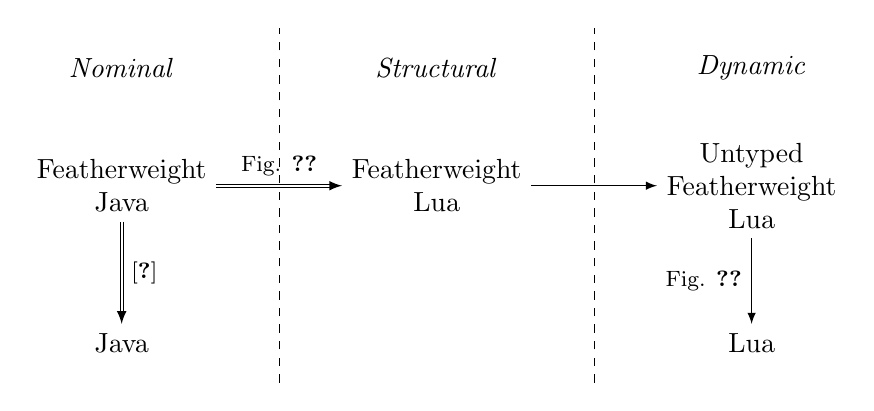
\begin{tikzpicture}
        \node[align=center] at (-4,  0) (fj) {Featherweight \\ Java};
        \node[align=center] at ( 0,  0) (fl) {Featherweight \\ Lua};
        \node[align=center] at ( 4,  0) (ufl) {Untyped \\ Featherweight \\ Lua};
        \node at (-4, -2) (java) {Java};
        \node at ( 4, -2) (lua) {Lua};
        \node at (-4, 1.5) (nominal) {\emph{Nominal}};
        \node at ( 0, 1.5) (structural) {\emph{Structural}};
        \node at ( 4, 1.5) (dynamic) {\emph{Dynamic}};
        \draw[-latex, double] (fj) -- (fl) node[midway,above] {\footnotesize Fig. \ref{fig:translation}}; 
        \draw[-latex, double] (fj) -- (java) node[midway,right] {\footnotesize \cite{featherweight-java}};
        \draw[-latex] (fl) -- (ufl);
        \draw[-latex] (ufl) -- (lua) node[midway,left] {\footnotesize Fig. \ref{fig:featherweight-lua-embedding}};
        \draw[dashed] (-2, -2.5) -- (-2, 2);
        \draw[dashed] (2, -2.5) -- (2, 2);
    \end{tikzpicture}
    \caption{Diagram depicting a scale of nominal, structural, and dynamic typing, with languages connected by translations between them. Its core is the translation of Featherweight Java (nominal) into Featherweight Lua (structural) from Section \ref{sec:translations}. Double arrows $\Rightarrow$ are translations that preserve both types and semantics, single arrows $\to$ only preserve semantics.}
    \label{fig:nominal-structural-dynamic}
\end{figure}

\section{Summary}

I have identified \textbf{duck typing} as a well-behaved pattern in dynamically typed programs, and \textbf{structural subtyping} as its appropriate model suitable for constructing expressive static type systems. I motivate this choice by presenting translations and embeddings for a pair of calculi: the nominally typed Featherweight Java, and the structurally typed Featherweight Lua. These formally reinforce intuitive beliefs about the static-dynamic and nominal-structural axes of type systems, and serve as groundwork for the thesis.

Though this dissertation does not explore the application of structural subtyping to statically typing \emph{specific} dynamic languages (e.g.\@ as part of a \emph{gradual} type system \cite{gradual-typing-for-objects}), it contributes elements of a framework for doing so and motivates the application of structural subtyping for this purpose. In the next chapter, we develop a general type inference framework for languages featuring structural subtyping -- including Featherweight Lua.

% It has by now become evident that the aim of this thesis is not to implement a new system for typing dynamic languages directly. Instead, I identify and develop general approaches that show potential to be used for this purpose. Furthermore, they can inform the design of (possibly domain-specific) languages that can admit more flexible type systems.